\documentclass[a4paper, 20pt,reqno]{article}
\usepackage[left=2cm,right=2cm,top=2cm,bottom=2cm]{geometry}
\usepackage[T2A]{fontenc}
% \DeclareMathSizes{10}{10}{10}{10}

\usepackage[russian]{babel}
\usepackage{soul}
\usepackage{gensymb}
\usepackage{amsfonts,amsmath,amssymb}
\usepackage{mathrsfs}
\usepackage{graphicx}
\usepackage[normalem]{ulem}
\usepackage[document]{ragged2e}
\usepackage{stmaryrd}
\usepackage{wrapfig}
\usepackage{fancyhdr}
\usepackage{floatflt}
\usepackage{python}
\usepackage{float}
\usepackage{amssymb}
\usepackage[most]{tcolorbox}
\usepackage{indentfirst}
\usepackage{setspace}
\usepackage{scrextend}
\usepackage{listings}
\usepackage{makecell,tabularx}
\usepackage{hyperref}
\usepackage{xcolor}

\newcommand{\mycopyright}{pluttan}
\newcommand{\docopyright}{$\mathfrak{Copyright}\ \mathfrak{\mycopyright} \logo$}
\newcommand{\rub}{{\rm{Р}\kern-.635em\rule[.5ex]{.52em}{.04em}\kern.11em}}

\definecolor{linkcolor}{HTML}{000000} 
\definecolor{urlcolor}{HTML}{0000FF} 

\hypersetup{pdfstartview=FitH,  linkcolor=linkcolor,urlcolor=urlcolor, colorlinks=true}

\definecolor{grey}{RGB}{40, 40, 40}

\renewcommand{\href}[1]{\url{#1}}

\definecolor{codegreen}{rgb}{0,0.6,0}
\definecolor{codegray}{rgb}{0.5,0.5,0.5}
\definecolor{codepurple}{rgb}{0.7,0,0.82}
\definecolor{mermaid}{rgb}{0.5,0.3,1}
\definecolor{backcolour}{rgb}{0.95,0.95,0.92}

\lstdefinestyle{mystyle}{
    backgroundcolor=\color{backcolour},   
    commentstyle=\color{codegreen},
    keywordstyle=\color{mermaid},
    numberstyle=\tiny\color{codegray},
    stringstyle=\color{codepurple},
    basicstyle=\ttfamily\footnotesize,
    breakatwhitespace=false,         
    breaklines=true,                 
    captionpos=b,                    
    keepspaces=true,                 
    numbers=left,                    
    numbersep=5pt,                  
    showspaces=false,                
    showstringspaces=false,
    showtabs=false,                  
    tabsize=2,
  extendedchars=true , % включаем не латиницу 
  escapechar=|, % |«выпадаем» в LATEX|
  frame=tb , % рамка сверху и снизу 
  commentstyle=\itshape , % шрифт для комментариев 
  stringstyle=\bfseries
}

\lstset{style=mystyle}

\lstdefinestyle{CommentStyle}{
    language=XML,
    %numbers=left, numberstyle=\tiny, stepnumber=1, numbersep=5pt,
    commentstyle=\color{red},
	basicstyle=\footnotesize\ttfamily,
	language={[ANSI]C++},
	keywordstyle=\bfseries,
	showstringspaces=false,
	morekeywords={include, printf},
	commentstyle={},
	escapeinside=§§,
	escapebegin=\begin{russian}\commentfont,
	escapeend=\end{russian},
    keywordstyle=\color{blue}\bfseries,
    morekeywords={align,begin},
    extendedchars=\true,
    tabsize=2
}
\lstdefinestyle{myLatexStyle}{
    language=c++,
    %backgroundcolor=\color{grey},
    numbers=left, numberstyle=\tiny, stepnumber=1, numbersep=5pt,
    commentstyle=\color{red},
    keywordstyle=\color{blue}\bfseries,
    morekeywords={align,begin},
    extendedchars=\true,
    tabsize=2
}

\lstdefinestyle{pmyLatexStyle}{
    language=java,
    %backgroundcolor=\color{grey},
    numbers=left, numberstyle=\tiny, stepnumber=1, numbersep=5pt,
    commentstyle=\color{red},
    keywordstyle=\color{blue}\bfseries,
    morekeywords={align,begin},
    extendedchars=\true,
    tabsize=2
}

\definecolor{block-gray}{gray}{0.90} % уровень прозрачности (1 - максимум)
\definecolor{yellow}{HTML}{F0FFFF}
\newtcolorbox{myquote}{colback=block-gray,grow to right by=-10mm,grow to left by=-10mm,boxrule=0pt,boxsep=0pt,breakable} % настройки области с изменённым фоном
\newtcolorbox{myquote2}{colback=yellow,grow to right by=-10mm,grow to left by=-10mm,boxrule=0pt,boxsep=0pt,breakable} % настройки области с изменённым фоном

\setlength{\parindent}{12,5mm}

\newcommand{\logo}{\vcenter{\hbox{
\includegraphics[width=.8em]{/Users/pluttan/Documents/bw2.png}}}}
\onehalfspacing

\pagestyle{fancy}
\renewcommand{\sectionmark}[1]{\markright{#1}}
\fancyhf{} 
\fancyhead[R]{\bfseries\thepage}
\fancyhead[LO]{\docopyright}

\newcommand{\image}[2]{
	\begin{figure}[H]
		\center{\includegraphics[height=#2pt]{../img/#1} }
    \end{figure}
}

\newcommand{\dotitle}[2]{

\thispagestyle{empty}
\sloppy{
  \scriptsize{
    \line(6,0){0}

    \centering \docopyright

    \centering Привет! Меня зовут Андрей, я создаю свою ботву, этот файл малая ее часть. 
    
    \centering Пользоваться и распространять файлы конечно же можно. Если вы нашли ошибку в файле, можете 
    
    \centering исправить ее в исходном коде и подать на слияние или просто написать в issue. 

    \centering {\bf{Так же вы можете купить распечатанную версию данного файла в виде книжки.}
    
    \centering По всем вопросам писать в ВК.}
    
    \centering Приятного бота)

    \line(6,0){300}

    \centering GitHub: \href{https://github.com/pluttan}

    \centering VK: \href{https://vk.com/pluttan}

    \line(6,0){0}
  }}

\begin{figure}[H]
		\center{\includegraphics[height=100pt]{/Users/pluttan/Documents/forMyDocs/qr2.png} }
\end{figure}

\topskip=-200pt
\vspace*{130pt}
\begin{Huge}
  \textbf{
    \begin{center}
        #1
    \end{center}
  }
  {\begin{center} 
        #2
    \end{center}}
\end{Huge}
\vspace*{300pt}
  \begin{flushright}
    Над файлом работали: \\
    \mycopyright
  \end{flushright}
\newpage
\pagestyle{fancy}
\renewcommand{\sectionmark}[1]{\markright{#1}}
\fancyhf{} 
\fancyhead[R]{\bfseries\thepage}
\fancyhead[LO]{\docopyright}
}
\renewcommand{\sectionmark}[1]{\markright{#1}}
\renewcommand{\sectionmark}[1]{\markright{#1}}
% \makeatletter
%      \renewcommand*\l@section{\@dottedtocline{1}{0em}{1.8em}}
%      \renewcommand*\l@subsection{\@dottedtocline{2}{1.5em}{2.0em}}
%      \renewcommand*\l@subsubsection{\@dottedtocline{3}{4.3em}{3.0em}}
% \makeatother
\newcommand{\toc}{
\newpage
\renewcommand{\contentsname}{Оглавление}
\large{\tableofcontents}
\newpage
\large
}


% It's XeLaTeX, if you can't compile comment this line 
\usepackage{fontspec}\setmainfont{Times New Roman} 

\renewcommand{\copyright}{fiixii, pluttan}

% \usepackage{titlesec}
% \titleformat{\section}
%   {\fontsize{18}{15}\bfseries}{\thesection}{1em}{}
% \titleformat{\subsection}
%   {\tt\fontsize{16}{15}\bfseries}{\thesubsection}{1em}{}

\newcommand{\hlek}[1]{{\normalsize\begin{center}\textit{Л.С. Сеченкова, Н.В. Палий Начертательная геометрия Лекционная тетрадь стр. #1}\end{center}}}
\newcommand{\hbook}[1]{{\normalsize\begin{center}\textit{Б.Г. Жирных, В.И. Серегин, Ю.Э. Шарикян Начертательная геометрия стр. #1}\end{center}}}


% It's XeLaTeX, if you can't compile:
% 1. download & install this https://isopromat.ru/wp-content/uploads/fonts-GOST.zip
% 2. try to use XeLaTeX 
% OR comment this line 

%%%%%%%%%%%%%%%%%%%%%%%%%%%%%%%%%%%%%%%%%%%%%%%%%%%%%%%%%%%%%%%%
%значения комментариев
%! Forced transition - вынужденный переход на новую страницу
%%%%%%%%%%%%%%%%%%%%%%%%%%%%%%%%%%%%%%%%%%%%%%%%%%%%%%%%%%%%%%%%
\begin{document}
%\setmonofont{GOST Type BU}
\setmainfont{GOST 2.304}
\tikz[remember picture,overlay] \node[opacity=0.1,inner sep=0pt] at (current page.center){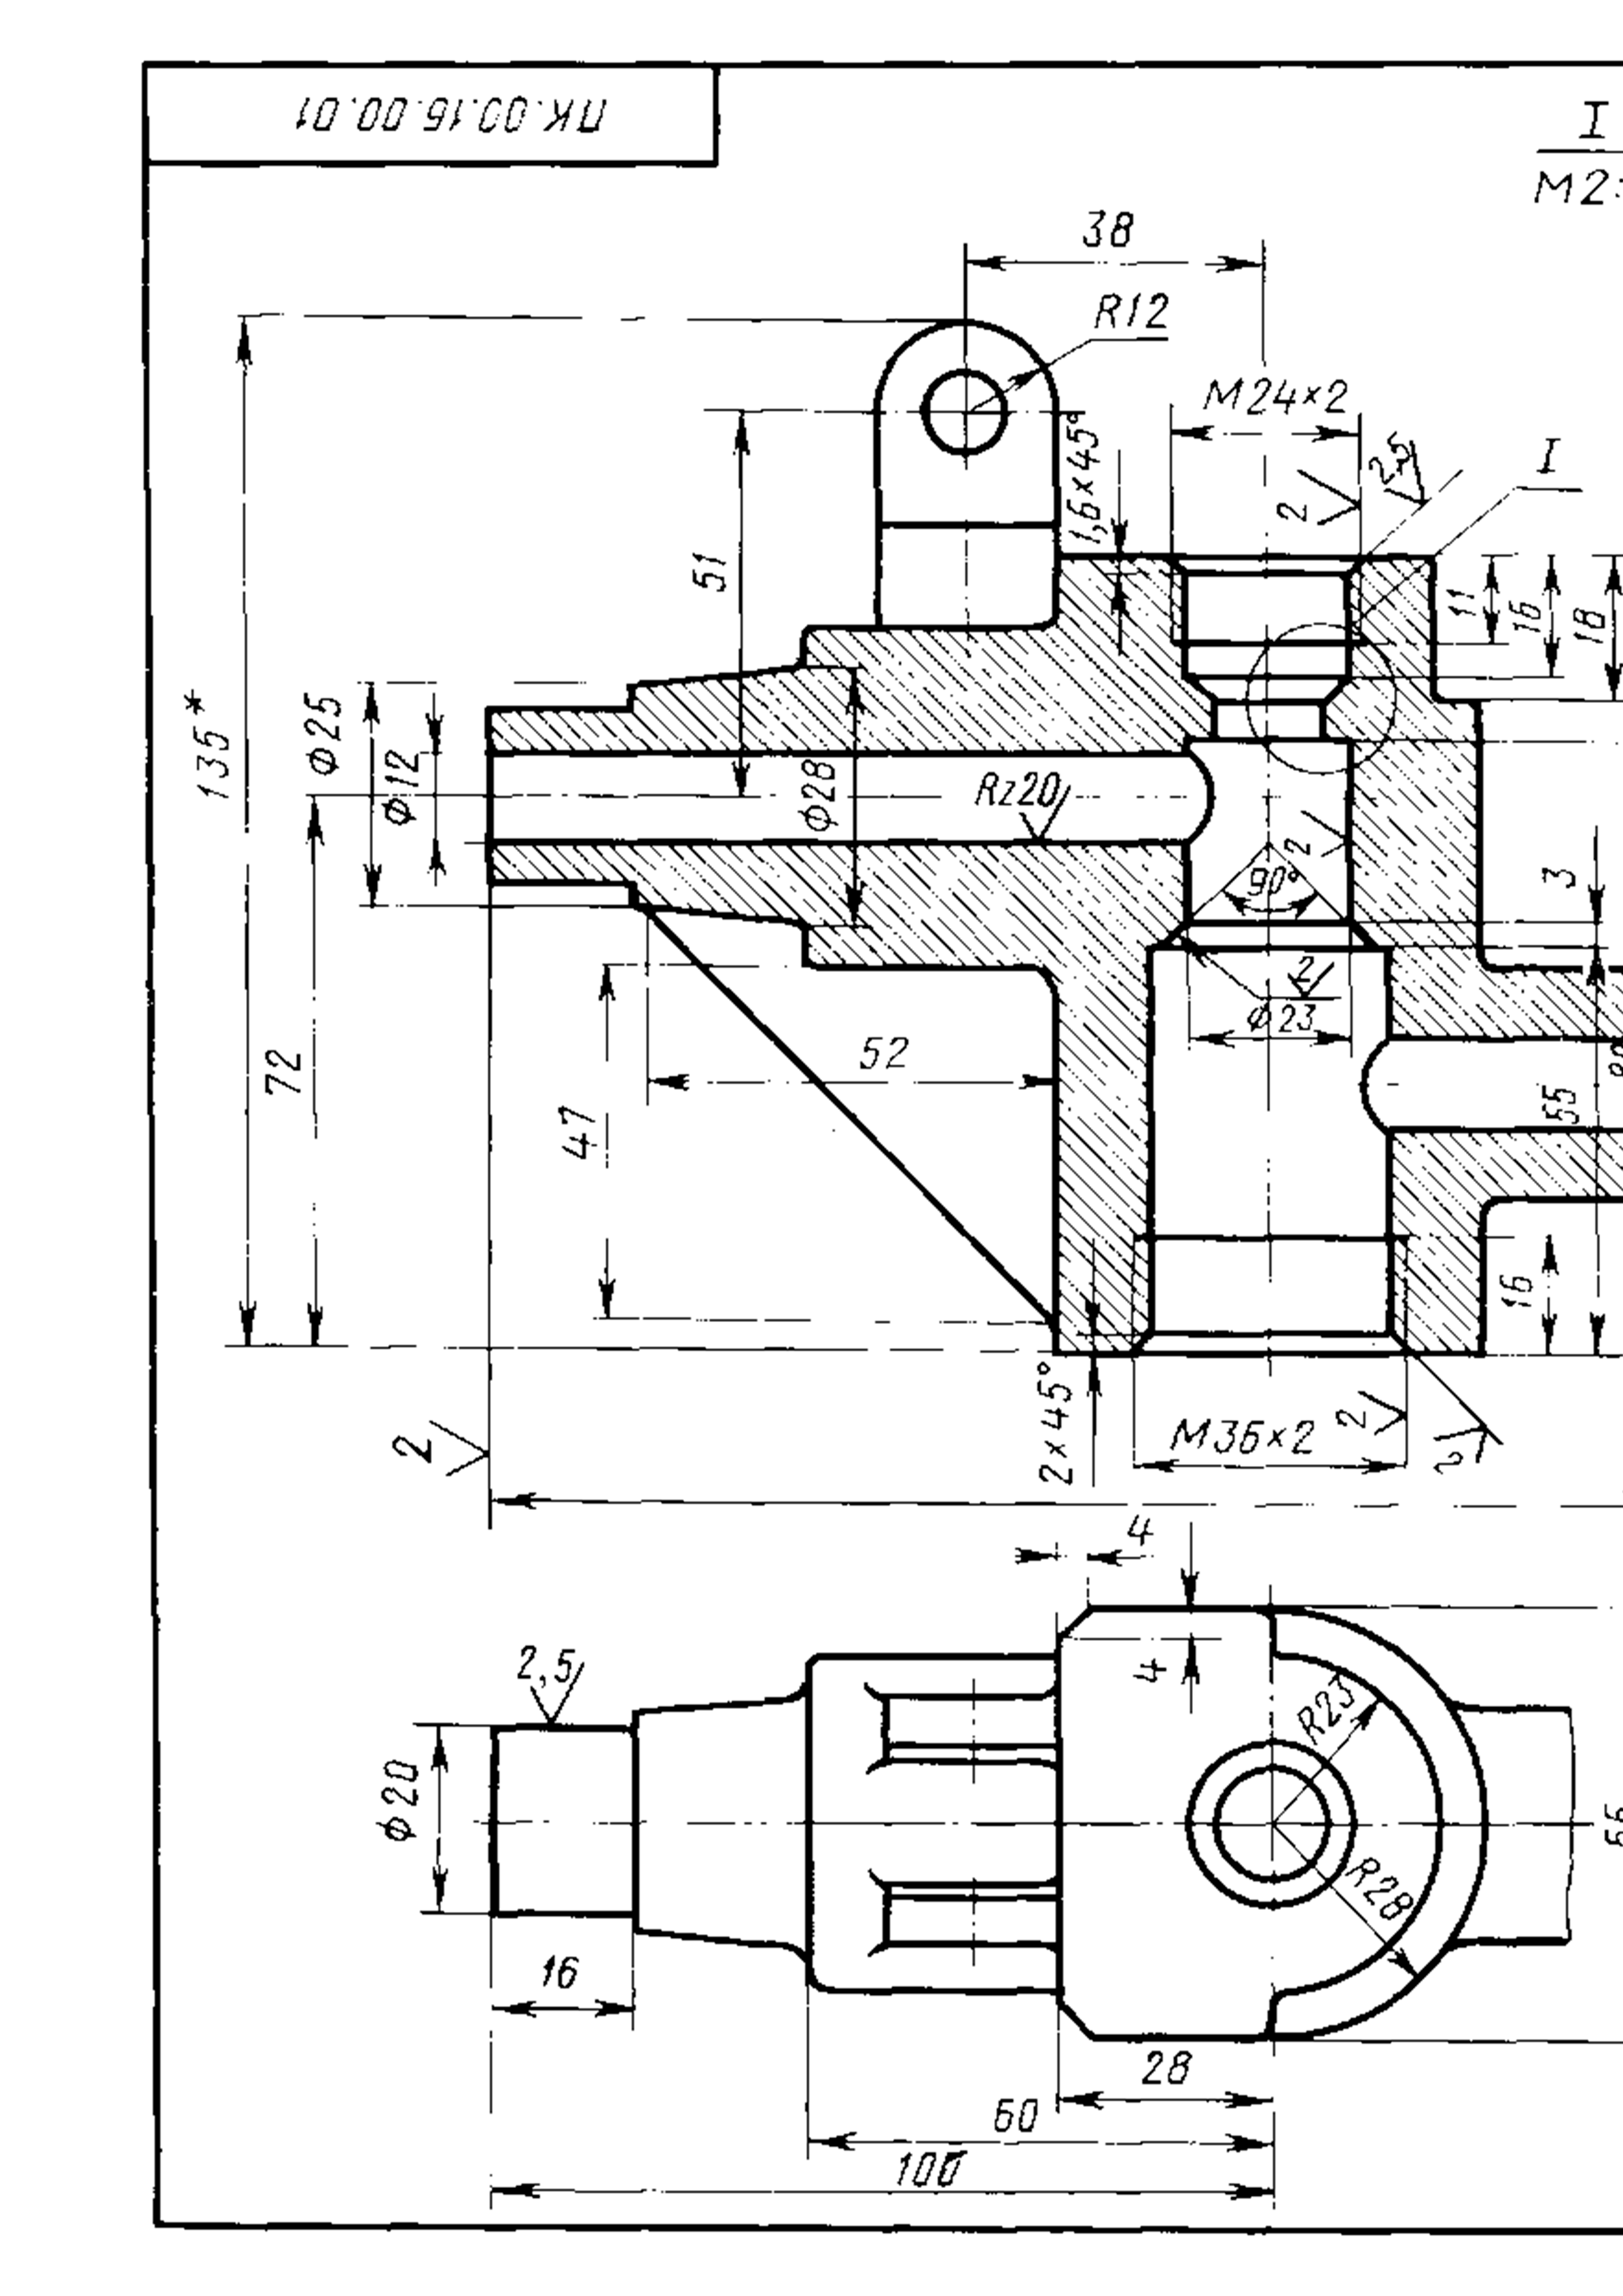
\includegraphics[width=\paperwidth,height=\paperheight]{../img/bg2.png}};
\dotitle{\textit{Подготовка к экзамену}}{\textit{Начертательная геометрия}}{}
\toc



\section*{\textbf{Инженерная графика}}\addcontentsline{toc}{section}{\textbf{Инженерная графика}}
\subsection*{1. \textit{Как расшифровывается аббревиатура ЕСКД?}}\addcontentsline{toc}{subsection}{1. \textit{Как расшифровывается аббревиатура ЕСКД?}}

\textbf{ЕСКД} - единая система конструкторской документации - комплекс государственных стандартов, устанавливающих правила, требования и нормы по разработке, оформлению и обращению конструкторской документации, разрабатываемой и применяемой на всех стадиях жизненного цикла изделия.
\subsection*{2. \textit{Обозначение основных форматов. Каково отношение сторон основных форматов?}}\addcontentsline{toc}{subsection}{2. \textit{Обозначение основных форматов. Каково отношение сторон основных форматов?}}
\begin{center}
\begin{tabular}{|c|c|c|c|c|c|c|}
\hline




Обозначение формата&A0&A1&A2&A3&A4&A5\\ \hline

Размеры сторон, мм &$841\times 1189$&$594\times 841$&$420\times 594$&$297\times 420$&$210\times 297$&$148\times 210$\\ \hline

\hline
\end{tabular}
\end{center}
\subsection*{3. \textit{Что называют масштабом изображения?}}\addcontentsline{toc}{subsection}{3. \textit{Что называют масштабом изображения?}}

\textbf{Масштабом} называется отношение линейных размеров изображения детали к действительным разерам изображаемой детали.
\subsection*{4. \textit{Ряд масштабов уменьшения и увеличения.}}\addcontentsline{toc}{subsection}{4. \textit{Ряд масштабов уменьшения и увеличения.}}
\begin{center}
\begin{tabular}{|c|c|c|c|c|c p{-10pt}|}
\hline




Масштабы уменьшения&$1:2$&$1:2,5$&$1:4$&$1:5$&$1:10$&\\ \hline

Масштаб натуральной величины&\multicolumn{5}{c}{$1:1$}&\\ \hline

Масштабы увеличения&$2:1$&$2,5:1$&$4:1$&$5:1$&$10:1$&\\ \hline

\hline
\end{tabular}
\end{center}
\subsection*{5. \textit{Как указывают масштаб на чертеже?}}\addcontentsline{toc}{subsection}{5. \textit{Как указывают масштаб на чертеже?}}

Масштаб указывается в предназначенной для этого графе основной надписи чертежа. Обозначается по типу $1:1$; $1:2$; $2:1$ и т.д.
\subsection*{6. \textit{Назначение основной сплошной толстой линии, сплошной тонкой линии, штрихпунктирной линии, штриховой линии. Указать параметры этих линий.}}\addcontentsline{toc}{subsection}{6. \textit{Назначение основной сплошной толстой линии, сплошной тонкой линии, штрихпунктирной линии, штриховой линии. Указать параметры этих линий.}}

\textbf{Основная сплошная толстая линия} - применяется для изображения видимого контура предмета, линий пересечения поверхностей и контура сечения (вынесенного или входящего в состав разреза).

\textbf{Сплошная тонкая линия} - применяется для изображения линий построения, выносных и размерных линий, а также для: линий контура наложенного сечения, линий-выносок, шриховки сечений.

\textbf{Штрихпунктирная линия} - применяется для изображения осевых и центровых линий.

\textbf{Штриховая линия} - применяется для изображения линий невидимого контура.


\image{img/6.jpg}{140}

\vspace{14pt} 
\begin{center}
\begin{tabular}{|c|c|}
\hline




Основная сплошная толстая линия&$s\ (0,6 - 1,5\text{мм})$\\ \hline

Сплошная тонкая линия&От $s/3$ до $s/2$\\ \hline

Штрихпунктирная линия&От $s/2$ до $2s/3$\\ \hline

Штриховая линия&От $s/3$ до $s/2$\\ \hline

\hline
\end{tabular}
\end{center}
% (0\_0) 
\subsection*{7. \textit{Ряд размеров шрифта. Каким размером букв определяется размер шрифта?}}\addcontentsline{toc}{subsection}{7. \textit{Ряд размеров шрифта. Каким размером букв определяется размер шрифта?}}

Устанавливаются следующие размеры шрифта:
\begin{center}
\begin{tabular}{|c|c|c|c|c|c|c|c|c|c|c|}
\hline




$1,8$мм&$2,5$мм&$3,5$мм&$5$мм&$7$мм&$10$мм&$14$мм&$20$мм&$28$мм&$40$мм\\ \hline

\hline
\end{tabular}
\end{center}

Размер шрифта определятся высотой прописных (заглавных) букв в мм.
\subsection*{8. \textit{Какое изображение называется видом?}}\addcontentsline{toc}{subsection}{8. \textit{Какое изображение называется видом?}}

\textbf{Видом} называется изображение, на котором показана обращенная к наблюдателю видимая часть поверхности предмета.
\subsection*{9. \textit{Как называются виды, получаемые на основных плоскостях проекций? Как располагают на чертеже основные виды?}}\addcontentsline{toc}{subsection}{9. \textit{Как называются виды, получаемые на основных плоскостях проекций? Как располагают на чертеже основные виды?}}


\image{img/9.jpg}{200}

\subsection*{10. \textit{Какое изображене предмета на чертеже принимают в качестве главного? Какие к нему требования?}}\addcontentsline{toc}{subsection}{10. \textit{Какое изображене предмета на чертеже принимают в качестве главного? Какие к нему требования?}}

Изображение на фронтальной плоскости проекций принимается на чертеже в качестве {\bf главного}. Главный вид должен давать наиболее полное представление о форме и размерах детали.

\subsection*{11. \textit{Какое изображение называют дополнительным видом, местным видом?}}\addcontentsline{toc}{subsection}{11. \textit{Какое изображение называют дополнительным видом, местным видом?}}

\textbf{Дополнительный вид} - получается проецированием предмета на плоскость, не параллельную ни одной из основных плоскостей проекций. Применяется в тех случаях, когда изображение предмета или его элемента не может быть показано на основных линиях без искажения формы и размеров.

\textbf{Местный вид} - изображение отдельного, ограниченного места поверхности предмета. Применяется в тех случаях, когда из всего вида только часть его необходима для уточнения формы предмета.
\subsection*{12. \textit{Какое изображение называется разрезом?}}\addcontentsline{toc}{subsection}{12. \textit{Какое изображение называется разрезом?}}

\textbf{Разрезом} называется изображение предмета, полученное при мысленном рассечении его одной или несколькими секущими плоскостями. При этом часть предмета, расположенная между наблюдателем и секущей плоскостью, мысленно удаляется, а на плоскости проекций изображается то, что получается в секущей плоскости и что расположено за ней.
\subsection*{13. \textit{Как обозначают разрезы на чертежах в общем случае?}}\addcontentsline{toc}{subsection}{13. \textit{Как обозначают разрезы на чертежах в общем случае?}}

Положение секущей плоскости указывается разомкнутой линией. Штрихи разомкнутой линии не должны пересекать контур детали. На штрихах разомкнутой линии перпендикулярно к ним ставят стрелки, указывающие направления взгляда. Около каждой стрелки наносится одна и та же прописная буква.


\image{img/13\_1.jpg}{210}


Надпись над разрезом содержит две буквы, которыми обозначена секущая плоскость, написанные через тире.

Фигура сечения предмета заштриховывается тонкими линиями под углом $45^{\circ}$ (если при этом линии штриховки параллельны линиям контура предмета или осевым линиям, то допускаются углы $30^{\circ}$ и $60^{\circ}$). Их наклон может выполняться влево или вправо, но в одну сторону на всех сечениях, относящихся к одной и той же детали.


\image{img/13\_2.jpg}{260}

\subsection*{14. \textit{В каких случаях не указывают положение секущей плоскости при выполнении разреза?}}\addcontentsline{toc}{subsection}{14. \textit{В каких случаях не указывают положение секущей плоскости при выполнении разреза?}}

В случаях, когда \textbf{секущая плоскость совпадает с плоскостью симметрии предмета}, не указывают положение секущей плоскости при выполнении разреза.
\subsection*{15. \textit{Как называются разрезы, расположенные на месте соответствующих видов?}}\addcontentsline{toc}{subsection}{15. \textit{Как называются разрезы, расположенные на месте соответствующих видов?}}

\textbf{Горизонтальные разрезы} (секущая плоскость параллельна горизонтальной плоскости проекций), \textbf{фронтальные разрезы} (секущая плоскость параллельна фронтальной плоскости проекций) и \textbf{профильные разрезы} (секущая плоскость параллельна профильной плоскости проекций) могут размещаться на месте соответствующих основных видов.
\subsection*{16. \textit{Как разделяются разрезы в зависимости от числа секущих плоскостей?}}\addcontentsline{toc}{subsection}{16. \textit{Как разделяются разрезы в зависимости от числа секущих плоскостей?}}

\textbf{Простые разрезы} - разрезы, образованные одной секущей плоскостью.


\image{img/c16\_1.jpg}{150}


\textbf{Сложные разрезы} - разрезы, образованные двумя и более секущими плоскостями.


\image{img/c16\_2.png}{180}

\subsection*{17. \textit{Какие линии являются разделяющими при соединении части вида и части соответствующего разреза?}}\addcontentsline{toc}{subsection}{17. \textit{Какие линии являются разделяющими при соединении части вида и части соответствующего разреза?}}

Для соединения части вида и части разреза используются:
\begin{itemize}

\item Штрихпунктирные (осевые)


\image{img/c17\_1.png}{200}

\item Сплошные волнистые - если с границей части вида и разреза совпадает линия контура.


\image{img/c17\_2.png}{200}


\end{itemize}
\subsection*{18. \textit{Как показывают на разрезе тонкие стенки типа ребер жесткости, если секущая плоскость направлена вдоль их длинной стороны?}}\addcontentsline{toc}{subsection}{18. \textit{Как показывают на разрезе тонкие стенки типа ребер жесткости, если секущая плоскость направлена вдоль их длинной стороны?}}

Тонкие стенки типа ребер жесткости показывают \textbf{незаштрихованными}, если секущая плоскость проходит вдоль длинной стороны элемента.


\image{img/c18.jpg}{150}

\subsection*{19. \textit{Какое изображение называют сечением? Какое сечение называют вынесенным, наложенным?}}\addcontentsline{toc}{subsection}{19. \textit{Какое изображение называют сечением? Какое сечение называют вынесенным, наложенным?}}

\textbf{Сечение} - ортогональная проекция фигуры, получающейся в одной или нескольких секущих плоскостях или поверхностях при мысленном рассечении проецируемого предмета. На сечении показывают только то, что находится непосредственно в секущей плоскости.

\textbf{Вынесенное сечение} - сечение, располагающееся на свободном поле чертежа.

\textbf{Наложенное сечение} - сечение, располагающееся непосредственно на изображении предмета.


\image{img/c19\_2.jpg}{250}

\subsection*{20. \textit{Какие сечения не обозначают на чертеже?}}\addcontentsline{toc}{subsection}{20. \textit{Какие сечения не обозначают на чертеже?}}

При выполнении \textbf{вынесенных} и \textbf{наложенных симметричных} сечений положение секущей плоскости не указывается.
\subsection*{21. \textit{В каких случаях сечение следует заменять разрезом?}}\addcontentsline{toc}{subsection}{21. \textit{В каких случаях сечение следует заменять разрезом?}}

Если сечение получается состоящим из отдельных частей, то сечение должно быть заменено разрезом.


\image{img/c21.png}{180}

\subsection*{22. \textit{Как графически на чертежах обозначают материалы в сечениях, на разрезах?}}\addcontentsline{toc}{subsection}{22. \textit{Как графически на чертежах обозначают материалы в сечениях, на разрезах?}}

Материалы в сечениях и разрезах обозначают с помощью разных типов штриховки.


\image{img/c22.jpg}{250}

\subsection*{23. \textit{Как выбирают направление линий штриховки и расстояние между ними для разных изображений одного и того же предмета на чертеже?}}\addcontentsline{toc}{subsection}{23. \textit{Как выбирают направление линий штриховки и расстояние между ними для разных изображений одного и того же предмета на чертеже?}}

Линии штриховки должны проводиться под углом $45^{\circ}$ (если при этом линии штриховки параллельны линиям контура предмета или осевым линиям, то допускаются углы $30^{\circ}$ и $60^{\circ}$). Их наклон может выполняться влево или вправо, но в одну сторону на всех сечениях, относящихся к одной и той же детали.

Расстояния между линиями штриховки должны быть одинаковыми для всех выполняемых в одном и том же масштабе сечений данной детали. Это расстояние выбирается от $1$ до $10 \text{мм}$, в зависимости от площади штриховки: большее расстояние соответствует большей площади фигуры сечения.
\subsection*{24. \textit{Чему равно минимальное растояние между размерной линией и линией контура изображения, между параллельными размерными линиями?}}\addcontentsline{toc}{subsection}{24. \textit{Чему равно минимальное растояние между размерной линией и линией контура изображения, между параллельными размерными линиями?}}

Минимальное расстояние между параллельными размерными линиями составляет $7$мм, а между размерной линией и линией контура - $10$мм.
\subsection*{25. \textit{В каких единицах измерения указывают размеры на чертежах?}}\addcontentsline{toc}{subsection}{25. \textit{В каких единицах измерения указывают размеры на чертежах?}}

Линейные размеры принято наносить в миллиметрах без указания единицы измерения. Если на чертеже нужно указать размеры не в мм, а в других единицах измерения, то соответствующие размерные числа записывают с обозначением единицы измерения.

\newpage

\section*{Начертательная геометрия}\addcontentsline{toc}{section}{\textbf{Начертательная геометрия}}

%-------------------------
%       Вопрос 1
%-------------------------

\subsection*{1. \textit{Свойства прямоугольного проецирования}}
\addcontentsline{toc}{subsection}{1. \textit{Свойства прямоугольного проецирования}}

\begin{mainQuote}
    \hlek{6}
    
    \hbook{16 - 20}
\end{mainQuote}

\begin{enumerate}
    \item Проекция точки есть точка.% ебнешься, да?)

    \image{img/1Point.jpg} {150}

    \item В общем случае проекция прямой есть прямая линия, проекция кривой линии есть кривая.

    \item Свойство принадлежности: при проецировании сохраняется принадлежность точки $A$ линии $l$: если $A \in l$, то $A' \in l'$.

    \image{img/1Property2.jpg} {150}

    \item Параллельные прямые проецируются в парралельные прямые.

    \image{img/1Property3.jpg} {150}
    \item Сохраняется простое отношение трех точек, т.е. {\Large $\frac{AB}{BC} = \frac{A'B'}{B'C'}$}.

    \image{img/1property5.jpg} {150}

\end{enumerate}


Для выполнения чертежей важно отметить следующие свойства:

\begin{enumerate}
    \item Если плоская фигура параллельна плоскоскости проекций, то она проецируется на эту плоскость без искажений.
    
    \image{img/1property2_2.jpg}{150}
    
    \item При параллельном переносе плоскости проекций в направлении проецирования проекции фигуры остаются неизменными.
    
\end{enumerate}

%-------------------------
%       Вопрос 2
%-------------------------

\newpage
\subsection*{2. \textit{Какие линии называются проецирующими линиями, линиями уровня?}}
\addcontentsline{toc}{subsection}{2. \textit{Какие линии называются проецирующими линиями, линиями уровня?}}

\begin{mainQuote}
    \hlek{8 - 9}
    
    \hbook{28 - 30}
\end{mainQuote}

Прямые, перпендикулярные плоскостям проекций, называются {\bf проецирующими}. Такие прямые проецируются в точку на ту плоскость проекций, которой эта
прямая перпендикулярна.

Выделяют следующие виды проецирующих прямых:
\begin{enumerate}
    \item \textit {Горизонтально-проецирующая прямая} (прямая, перпендикулярная горизонтальной плоскости проекций).
    
    \image{img/2Horisontal.jpg}{150}

    \item \textit{Фронтально-проецирующая прямая} (прямая, перпендикулярная фронтальной плоскости проекций).

    \image{img/2Frontal.jpg}{150}

    \item \textit {Профильно-проецирующая прямая} (прямая, перпендикулярная профильной плоскости проекций).

    \image{img/2Profile.jpg}{150}

\end{enumerate}


Прямые, параллельные плоскостям проекций, называются {\bf прямыми
уровня}.

Выделяют следующие виды прямых уровня:
\begin{enumerate}
    \item \textit {Горизонтальная прямая} (прямая, параллельная горизонтальной плоскости проекций).
    
    \image{img/2HorisontalPar.jpg}{150}

    \item \textit {Фронтальная прямая} (прямая, параллельная фронтальной плоскости проекций).

    \image{img/2FrontalPar.jpg}{150}

    \item \textit {Профильная прямая} (прямая, параллельная профильной плоскости проекций).

    \image{img/2ProfilePar.jpg}{150}

\end{enumerate}

%-------------------------
%       Вопрос 3
%-------------------------

\newpage
\subsection*{3. \textit{Какие линии, принадлежащие плоскости, называются горизонталью, фронталью?}}
\addcontentsline{toc}{subsection}{3. \textit{Какие линии, принадлежащие плоскости, называются горизонталью, фронталью?}}

\begin{mainQuote}
    \hlek{12 - 13}
    
    \hbook{46 - 48}
\end{mainQuote}

{\bf Горизонталью плоскости} называется прямая, принадлежащая данной плоскости и параллельная горизонтальной плоскости проекций.

\image{img/horisontal.png}{170}

{\bf Фронталью плоскости} называется прямая, принадлежащая данной плоскости и параллельная фронтальной плоскости проекций.

\image{img/frontal.png}{170}

%-------------------------
%       Вопрос 4
%-------------------------

\newpage
\subsection*{4. \textit{Теорема о проецировании прямого угла}}
\addcontentsline{toc}{subsection}{4. \textit{Теорема о проецировании прямого угла}}

\begin{mainQuote}
    \hlek{10}
\end{mainQuote}

Если одна сторона прямого угла параллельна плоскости проекций, а вторая сторона не перпендикулярна к ней, то прямой угол проецируется без искажения на данную плоскость проекций.

\image{img/4Teor.jpg}{250}

%-------------------------
%       Вопрос 5
%-------------------------

\newpage
\subsection*{5. \textit{На основании каких положений строят перпендикулярные: прямую и плоскость?}}
\addcontentsline{toc}{subsection}{5. \textit{На основании каких положений строят перпендикулярные: прямую и плоскость?}}

\begin{mainQuote}
    \hlek{14}
    
    \hbook{50}
\end{mainQuote}

Построение на чертеже {\bf перпендикулярных} прямой и плоскости основано на:

\begin{enumerate}
    \item Использовании \textit {признака перпендикулярности прямой и плоскости}: прямая перпендикулярна плоскости, если она перпендикулярна двум пересекающимся прямым, принадлежащим этой плоскости;
    \item Использовании \textit {теоремы о проекциях прямого угла}.
\end{enumerate}


%-------------------------
%       Вопрос 6
%-------------------------

\newpage
\subsection*{6. \textit{На основании каких положений строят параллельные: прямую и плоскость?}}
\addcontentsline{toc}{subsection}{6. \textit{На основании каких положений строят параллельные: прямую и плоскость?}}

\begin{mainQuote}
    \hlek{13}
    
    \hbook{49}
\end{mainQuote}

Построение на чертеже {\bf параллельных} прямой и плоскости основано на:

\begin{enumerate}
    \item Использовании \textit {признака параллельности прямой и плоскости}: прямая параллельна плоскости, если она параллельна прямой, принадлежащей этой плоскости;
    \item Использовании \textit {свойства проецирования параллельных прямых}: если прямые параллельны, то и проекции этих прямых параллельны.
\end{enumerate}



%-------------------------
%       Вопрос 7
%-------------------------

\newpage
\subsection*{7. \textit{На основании каких положений строят на чертеже две параллельные плоскости?}}
\addcontentsline{toc}{subsection}{7. \textit{На основании каких положений строят на чертеже две параллельные плоскости?}}

\begin{mainQuote}
    \hlek{14}
    
    \hbook{49}
\end{mainQuote}

Построение на чертеже {\bf параллельных} плоскостей основано на:

\begin{enumerate}
    \item Использовании \textit {признака параллельности двух плоскостей}: две плоскости параллельны, если две пересекающиеся прямые одной плоскости параллельны двум пересекающимся прямым другой плоскости;
    \item Использовании \textit {свойства проецирования параллельных прямых}: если прямые параллельны, то и проекции этих прямых параллельны.
\end{enumerate}

%-------------------------
%       Вопрос 8
%-------------------------

\newpage
\subsection*{8. \textit{На основании каких положений строят на чертеже две перпендикулярные плоскости?}}
\addcontentsline{toc}{subsection}{8. \textit{На основании каких положений строят на чертеже две перпендикулярные плоскости?}}

\begin{mainQuote}
    \hlek{15}
    
    \hbook{50 - 51}
\end{mainQuote}

Построение на чертеже {\bf перпендикулярных} плоскостей основано на:
\begin{enumerate}
    \item использовании \textit {признака перпендикулярности двух плоскостей}: две плоскости взаимно перпендикулярны, если одна из этих плоскостей содержит прямую, перпендикулярную к другой плоскости;
    \item использовании \textit {теоремы о проекциях прямого угла}.
\end{enumerate}



%-------------------------
%       Вопрос 9 
%-------------------------

\newpage
\subsection*{9. \textit{Правило построения проекции точки, принадлежащей поверхности}}
\addcontentsline{toc}{subsection}{9. \textit{Правило построения проекции точки, принадлежащей поверхности}}

\begin{mainQuote}
    \hlek{19}
\end{mainQuote}

Общее правило построения проекций точки, принадлежащей поверхности:

Для построения проекции точки, принадлежащей поверхности, надо воспользоваться проекциями линии, {\bf принадлежащей поверхности} и {\bf проходящей через заданную точку}. 

%-------------------------
%       Вопрос 10
%-------------------------

\newpage
\subsection*{10. \textit{Правило построения проекции точки, принадлежащей плоскости}}
\addcontentsline{toc}{subsection}{10. \textit{Правило построения проекции точки, принадлежащей плоскости}}

\begin{mainQuote}
    \hlek{12}
    
    \hbook{45}
\end{mainQuote}

Общее правило построения проекции точки, принадлежащей плоскости:

Для построения проекции точки, принадлежащей плоскости общего положения, надо воспользоваться проекциями прямой, {\bf принадлежащей заданной плоскости} и {\bf проходящей через заданную точку} (используем свойство принадлежности).


%-------------------------
%       Вопрос 11 %?check
%-------------------------

\newpage
\subsection*{11. \textit{Правило построения проекций точки, принадлежащей поверхности вращения}}
\addcontentsline{toc}{subsection}{11. \textit{Правило построения проекций точки, принадлежащей поверхности вращения}}

\begin{mainQuote}
    \centering Сформулировал $fiixii$
\end{mainQuote}

Общее правило построения проекций точки, принадлежащей поверхности вращения:

Для построения проекции точки, принадлежащей поверхности вращения, надо воспользоваться проекциями линии, {\bf являющейся образующей поверхности} и {\bf проходящей через заданную точку}. 

%-------------------------
%       Вопрос 12
%-------------------------

\newpage
\subsection*{12. \textit{Способы преобразования}}
\addcontentsline{toc}{subsection}{12. \textit{Способы преобразования}}

\begin{mainQuote}
    \hlek{24 - 32}
    
    \hbook{52 - 66}
\end{mainQuote}

Различают три способа преобразования:
\begin {enumerate}

\item {\bf Cпособ замены плоскостей проекций} - суть этого способа заключается в том, что в системе двух плоскостей проекций заменяют одну из плоскостей проекций на новую плоскость, перпендикулярную
неизменяемой плоскости проекций. На эту плоскость проецируют заданные
геометрические фигуры, которые в пространстве неподвижны.

\image{img/12ReplacePlanes.jpg}{140}

\item {\bf Cпособ плоскопараллельного перемещения} - суть этого способа заключается в том, что все точки геометрической фигуры перемещаются в
параллельных плоскостях.

\image{img/12ReplacePlanes2.jpg}{120}

\item {\bf Cпособ вращения (вокруг проецирующей прямой)} - суть этого способа заключается в том, что все точки фигуры движутся по окружностям в плоскостях, перпендикулярных к оси вращения (т.е. параллельно плоскости проекций, которой перпендикулярна ось вращения).

\image{img/12Rotation.jpg}{140}

\end {enumerate}



%-------------------------
%       Вопрос 13
%-------------------------

\newpage
\subsection*{13. \textit{Условия преобразования способом замены плоскостей проекций}}
\addcontentsline{toc}{subsection}{13. \textit{Условия преобразования способом замены плоскостей проекций}}

\begin{mainQuote}
    \hlek{24 - 27}
    
    \hbook{52 - 58}
\end{mainQuote}

Условия преобразования:
\begin{enumerate}
    \item Положение фигуры неизменно;
    \item Изменяется положение одной из двух плоскостей проекций;
    \item Новую плоскость проекций располагают перпендикулярно оставшейся плоскости проекций;
    \item Положение новой плоскости проекций может быть задано или выбрано.
\end{enumerate}

%-------------------------
%       Вопрос 14
%-------------------------

\newpage
\subsection*{14. \textit{Условия преобразования способом вращения вокруг проецирующей прямой}}
\addcontentsline{toc}{subsection}{14. \textit{Условия преобразования способом вращения вокруг проецирующей прямой}}

\begin{mainQuote}
    \hlek{29 - 32}
    
    \hbook{63 - 66}
\end{mainQuote}

Условия преобразования:
\begin{enumerate}
    \item Ось вращения i неподвижна и перпендикулярна плоскости проекций;
    \item Все точки фигуры перемещаются по окружностям, плоскости которых перпендикулярны оси i;
    \item Точки, лежащие на оси i, неподвижны.
\end{enumerate}

%-------------------------
%       Вопрос 15 
%-------------------------

\newpage
\subsection*{15. \textit{Какая линия поверхности вращения называется меридианом, параллелью?}}
\addcontentsline{toc}{subsection}{15. \textit{Какая линия поверхности вращения называется меридианом, параллелью?}}

\begin{mainQuote}
    \hlek{20}
\end{mainQuote}
{\bf Меридиан} - это линия пересечения поверхности вращения с плоскостью, проходящей через ось вращения (такая плоскость называется \textit {меридиональной}).

{\bf Главным меридианом} называют меридиан, лежащий в плоскости уровня.

{\bf Параллель} - это окружность, описываемая точкой, лежащей на образующей, при ее вращении вокруг оси вращения. 
\begin{itemize}
    \item Центр параллели лежит на оси вращения; 
    \item Параллель лежит в плоскости, перпендикулярной оси вращения.
\end{itemize}

Наибольшая параллель называется {\bf экватором}, наименьшая - {\bf горлом}.

\image{img/15_1.jpg}{200}

%-------------------------
%       Вопрос 16 %?check
%-------------------------

\newpage
\subsection*{16. \textit{В какую линию может проецироваться окружность при разных ее положениях отностельно плоскостей проекций?}}
\addcontentsline{toc}{subsection}{16. \textit{В какую линию может проецироваться окружность при разных ее положениях отностельно плоскостей проекций?}}

\begin{mainQuote}
    \hlek{17}
\end{mainQuote}
Окружность может проецироваться в:
\begin{itemize}
    \item {\bf окружность}, если плоскость проекции параллельна плоскости, в которой лежит окружность.
    \item {\bf прямую}, если плоскость проекции перпендикулярна плоскости, в которой лежит окружность.
    \item {\bf эллипс}, в остальных случаях.
\end{itemize}

\image{img/16_1.jpg}{250}

%-------------------------
%       Вопрос 17
%-------------------------

\newpage
\subsection*{17. \textit{Алгоритм построения точек пересечения линии с поверхностью}}
\addcontentsline{toc}{subsection}{17. \textit{Алгоритм построения точек пересечения линии с поверхностью}}

\begin{mainQuote}
    \hlek{39}
\end{mainQuote}
Алгоритм построения точек пересечения линии с поверхностью:
\begin{enumerate}
    \item заключить данную линию $a$ во вспомогательную поверхность $\gamma$;
    \item определить линию $l$ пересечения этой вспомогательной поверхности с заданной поверхностью;
    \item отметить точки, в которых пересекаются полученная линия $l$ с заданной линией $a$.
\end{enumerate}

\image{img/17_1.jpg}{150}
%-------------------------
%       Вопрос 18 %?check
%-------------------------

\newpage
\subsection*{18. \textit{Последовательность построения точки пересечения прямой и плоскости}}
\addcontentsline{toc}{subsection}{18. \textit{Последовательность построения точки пересечения прямой и плоскости}}

\begin{mainQuote}
    \hlek{40}
    \hbook{103}
\end{mainQuote}

Последовательность построения:
\begin{enumerate}
    \item заключаем данную прямую $a$ во вспомогательную проецирующую плоскость $\gamma$;
    \item строим проекции линии $l$ пересечения данной плоскости с плоскостью $\gamma$;
    \item строим проекции точки пересечения полученной линии $l$ с данной прямой $a$.
Полученная в последнем пункте точка - и есть точка пересечения прямой и плоскости.
\end{enumerate}

\image{img/18.jpg}{270}

%-------------------------
%       Вопрос 19
%-------------------------

\newpage
\subsection*{19. \textit{Последовательность построения точек пересечения прямой и поверхности}}
\addcontentsline{toc}{subsection}{19. \textit{Последовательность построения точек пересечения прямой и поверхности}}

\begin{mainQuote}
    \hlek{41 - 43}
    \hbook{131}
\end{mainQuote}

Последовательность построения:
\begin{enumerate}
    \item Данную прямую $a$ заключают во вспомогательную проецирующую плоскость $\gamma$.
    \item Строят линию $l$ пересечения вспомогательной плоскости $\gamma$ с заданной поверхностью.
    \item На пересечении построенной линии $l$ с данной прямой $a$ находят искомые точки.
\end{enumerate}



%-------------------------
%       Вопрос 20
%-------------------------

\newpage
\subsection*{20. \textit{Какие линии получаются в сечении цилиндрической поверхности плоскостью при разных положениях плоскости относительно оси цилиндрической поверхности?}}
\addcontentsline{toc}{subsection}{20. \textit{Какие линии получаются в сечении цилиндрической поверхности плоскостью при разных положениях плоскости относительно оси цилиндрической поверхности?}}

\begin{mainQuote}
    \centering Сформулировал $fiixii$
\end{mainQuote}

\begin{enumerate}
    \item Секущая плоскость {\bf параллельна} оси цилинда:
    \begin{itemize}
        
        \item Расстояние от оси до секущей плоскости {\bf меньше} радиуса основания цилиндра: в сечении будет {\bf две образующие};
        \image{img/20_1_1.jpg}{200}

        \item Расстояние от оси до секущей плоскости {\bf равно} радиусу основания цилиндра: в сечении будет {\bf одна образующая}; 
        \image{img/20_1_2.jpg}{200}

        \item Расстояние от оси до секущей плоскости {\bf больше} радиуса основания цилиндра: секущая плоскость {\bf не пересекает} цилиндр;

    \end{itemize}
    \item Секущая плоскость пересекает ось цилиндра под углом $\alpha (0\textdegree < \alpha \leqslant 90\degree)$
    \begin {itemize}

        \item Секущая плоскость {\bf параллельна} основаниям цилиндра: в сечении будет {\bf окружность};
        \image{img/20_2_1.jpg}{200}

        \item Секущая плоскость {\bf не пересекает ни одну окружность в основаниях цилиндра}: в сечении будет {\bf эллипс};
        \image{img/20_2_2.jpg}{200}

        \item Секущая плоскость {\bf пересекает минимум одно из оснований цилиндра}: в сечении будет {\bf часть эллипса};
        \image{img/20_2_3.jpg}{200}

    \end{itemize}
    
\end{enumerate}
%-------------------------
%       Вопрос 21
%-------------------------

\newpage
\subsection*{21. \textit{Конические сечения. При каком положении плоскости относительно оси конической поверхности сечением является окружность, эллипс, прямые, парабола, гипербола?}}
\addcontentsline{toc}{subsection}{21. \textit{Конические сечения. При каком положении плоскости относительно оси конической поверхности сечением является окружность, эллипс, прямые, парабола, гипербола?}}

\begin{mainQuote}
    \hlek{36}
\end{mainQuote}

\begin{enumerate}
    \item Секущая плоскость $\alpha$ {\bf не проходит через вершину конуса}:
    \begin{itemize}
        \item Секущая плоскость пересекает все образующие конуса и параллельна основанию: в сечении будет {\bf окружность};
        \image{img/n21_1_1.png}{190}
        \item Секущая плоскость пересекает все образующие конуса и не параллельна основанию: в сечении будет {\bf эллипс};
        \image{img/n21_1_2.png}{190}
        \item Секущая плоскость параллельна одной образующей конуса: в сечении будет {\bf парабола};
        \image{img/n21_1_3.png}{190}
        \item Секущая плоскость параллельна двум образующим конуса: в сечении будет {\bf гипербола}.
        \image{img/n21_1_4.png}{200}
    \end{itemize}
    \item Секущая плоскость $\alpha$ {\bf проходит через вершину конуса}:
    \begin{itemize}
        \item Угол между секущей плоскостью и осью вращения {\bf меньше} чем угол между образующей и осью вращения: в сечении будет {\bf две образующие};
        \image{img/n21_2_1.png}{200}
        \item Угол между секущей плоскостью и осью вращения {\bf равен} углу между образующей и осью вращения: в сечении будет {\bf одна образующая};
        \image{img/n21_2_2.png}{200}
        \item Угол между секущей плоскостью и осью вращения {\bf больше} чем угол между образующей и осью вращения: в сечении {\bf будет точка - вершина конуса};
        \image{img/n21_2_3.png}{200}

    \end{itemize}
\end{enumerate}


%-------------------------
%       Вопрос 22
%-------------------------

\newpage
\subsection*{22. \textit{Последовательность построения линии пересечения двух поверхностей}}
\addcontentsline{toc}{subsection}{22. \textit{Последовательность построения линии пересечения двух поверхностей}}

\begin{mainQuote}
    \hlek{43}
    \hbook{115 - 128}
\end{mainQuote}

\begin{enumerate}
    \item Вводим несколько вспомогательных параллельных плоскостей.
    \item Строим линии пересечения каждой введенной плоскости с каждой из поверхностей.
    \item Находим точки пересечения линий, построенных в предыдущем пункте, лежащих в одной вспомогательной плоскости.
    \item Проводим через полученные точки линию.
\end{enumerate}

%-------------------------
%       Вопрос 23
%-------------------------

\newpage
\subsection*{23. \textit{Теорема Монжа. Привести пример}}
\addcontentsline{toc}{subsection}{23. \textit{Теорема Монжа. Привести пример}}

\begin{mainQuote}
    \hlek{47}
    
    \hbook{127-128}
\end{mainQuote}

Если две поверхности второго порядка вписаны или описаны около третьей поверхности второго порядка, то они пересекаются по двум плоским кривым второго порядка. Плоские кривые проецируются в отрезки прямых линий на общую плоскость симметрии пересекающихся плоскостей. На чертеже эти отрезки прямых пересекаются в точке, которая является проекцией точек пересечения линий касания.

\image{img/23monz.jpg}{200}

%-------------------------
%       Вопрос 24
%-------------------------

\newpage
\subsection*{24. \textit{Какую плоскость называют касательной к поверхности в данной точке?}}
\addcontentsline{toc}{subsection}{24. \textit{Какую плоскость называют касательной к поверхности в данной точке?}}

\begin{mainQuote}
    \hlek{48}
    
    \hbook{137-139}
\end{mainQuote}

Плоскость, образованная касательными прямыми к двум любым линиям поверхности, пересекающимися в заданной на поверхности точке, называется {\bf касательной к поверхности в данной точке}.

\image{img/24kas.jpg}{200}

%-------------------------
%       Вопрос 25
%-------------------------

\newpage
\subsection*{25. \textit{Что называется нормалью к поверхности в данной точке?}}
\addcontentsline{toc}{subsection}{25. \textit{Что называется нормалью к поверхности в данной точке?}}

\begin{mainQuote}
    \hlek{48}
    
    \hbook{137-139}
\end{mainQuote}

{\bf Нормаль} $n$ к поверхности в данной точке перпендикулярна к касательной плоскости в этой точке поверхности.

\image{img/24kas.jpg}{200}

\newpage
\section*{\textbf{Новые вопросы}}\addcontentsline{toc}{section}{\textbf{Новые вопросы}}
\subsection*{1. \textit{Какие фигуры могут занимать проецирующее положение?}}\addcontentsline{toc}{subsection}{1. \textit{Какие фигуры могут занимать проецирующее положение?}}
\begin{mainQuote}
    \hlek{39}
\end{mainQuote}

\textbf{Прямая}, \textbf{плоскость} и \textbf{цилиндрическая поверхность} могут занимать проецирующее положение (т.е. положение, при котором фигура перпендикулярна одной из плоскостей проекций).

\vspace*{28pt}
\subsection*{2. \textit{По какой линии пересекаются соосные поверхности вращения?}}\addcontentsline{toc}{subsection}{2. \textit{По какой линии пересекаются соосные поверхности вращения?}}
\begin{mainQuote}
    \hlek{46}
    \hbook{124}
\end{mainQuote}

Две соосных поверхности вращения пересекаются по \textbf{общим параллелям} (окружностям, плоскости которых перпендикулярны оси вращения).
\image{img/huinakakauato.jpg}{180}


%для потомков ( Андрей старался :) )
%$\alpha$ - поверхность,
%$a \subset \alpha; b \subset \alpha; a \cub b \rightarrow A;$
%$t_1 \overline{\cup} a; t_2 \overline{\cup} a; t_1 \cap t_2 \rightarrow A; n \perp ( t_1 \cap t_2)$


\newpage
\let\clearpage\relax
\end{document}